\section{Introduction}\label{sec:introduction}
  \subsection{BGPStream}
 The exterior gateway protocol, Border Gateway Protocol (BGP) is used to exchange reachability information among routers in different autonomous systems. BGP is a path vector protocol and BGP routers send path vector messages to their neighbors to advertise the reachability information. These BGP messages enable the routers to construct an autonomous system (AS) connectivity graph and make routing policy decisions. BGP is a control plane protocol and governs how data plane forwards packets between autonomous systems. 
 \begin{figure}
	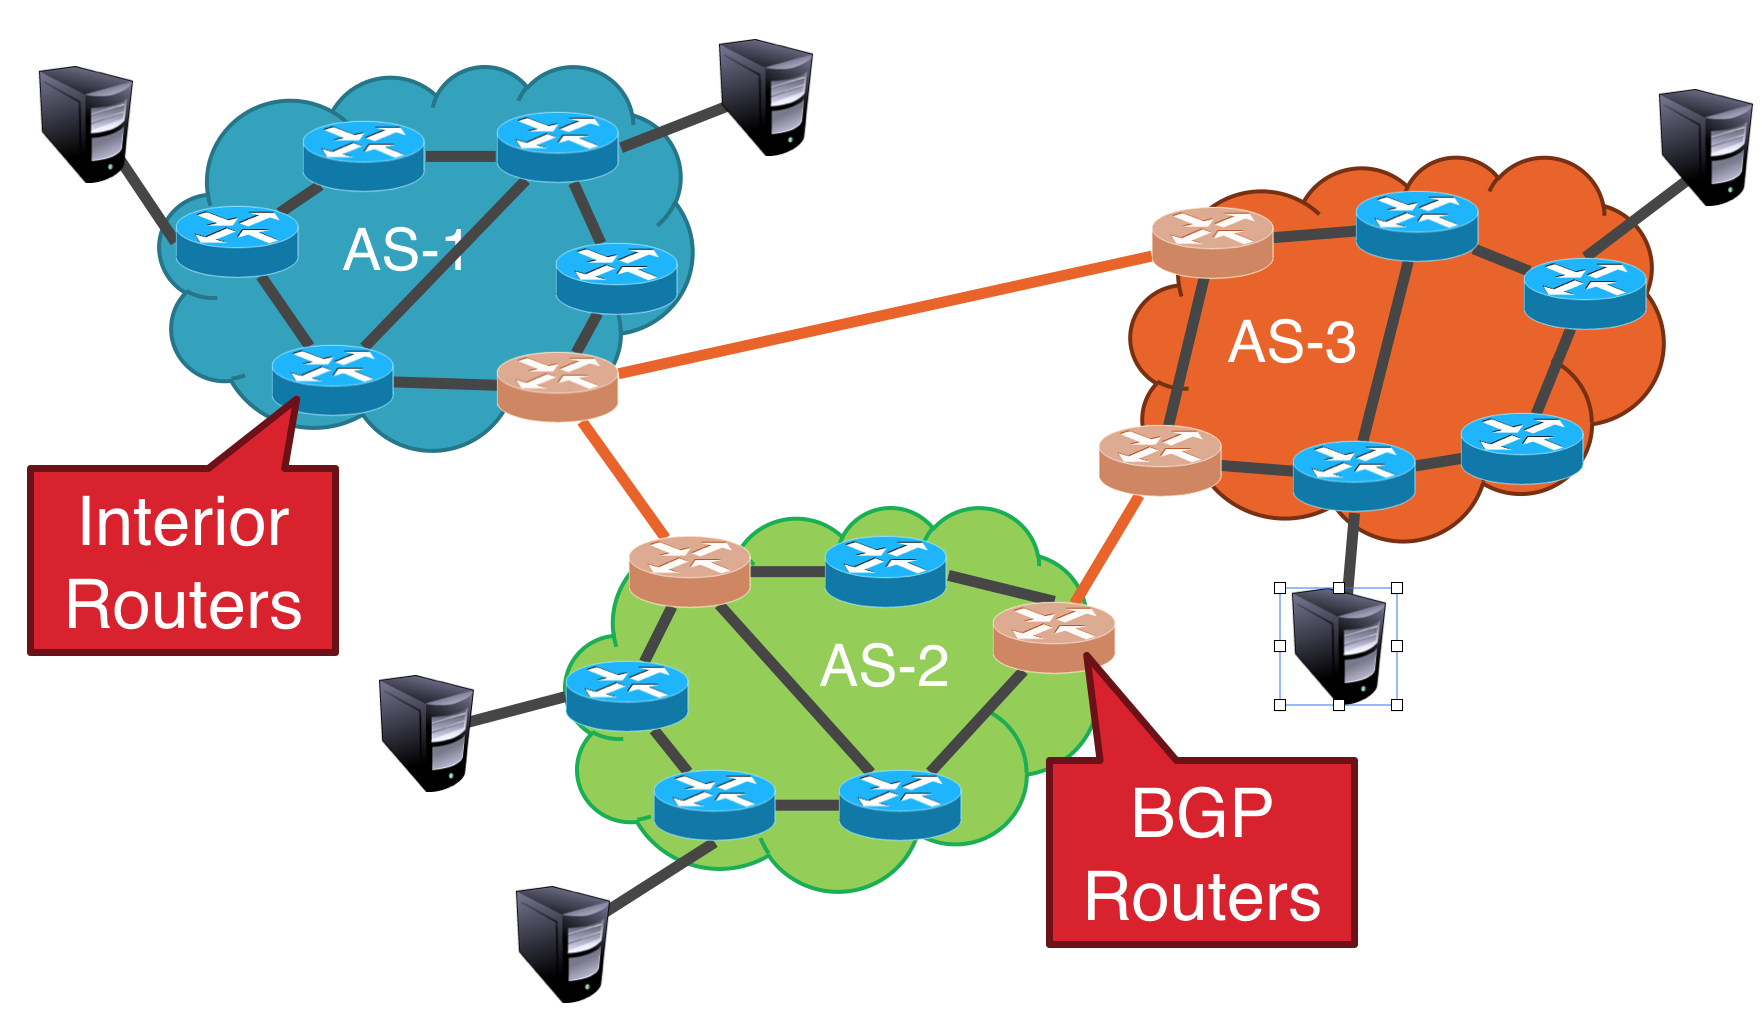
\includegraphics[width=0.5\textwidth]{Interior_and_BGP_routers.png}
	\caption{BGP routers are responsible for exchanging the path vector information. Interior routers run interior gateway protocol such as OSPF.}
\end{figure}
From the BGP routing table, a lot can be inferred about the internet topology and the peering agreements between different autonomous systems. BGP route monitors such as Route View, RIPE NCC, OpenBMP, BGPMon have made arrangements with some regional ISPs to get a dump of their RIB tables and updates to the tables. Route View monitors output RIB of participating ASes every two hours and RIPE outputs RIB every 8 hours\cite{orsini_bgpstream:_2016}. In addition to the RIB table, the monitors also output the updates to the routing table at a higher frequency. BGPStream provides a framework to analyze live and historical BGP data collected bu these monitors.  
\subsection{Anomalies in the BGP Data}
With the structure of the internet changing from hierarchical to flat, the pattern in which the autonomous systems announce prefixes has started to change. Multiple ASes announcing the same BGP prefix is no longer considered an anomaly. Emergence of CDNs has resulted in the same prefix being announced in different countries. Big organizations own multiple ASes hence, announce overlapping prefixes. Business relationships result in prefixes being traded among autonomous systems.\\
Multiple ASes announcing the same prefix can be due the changing structure of the internet, for traffic engineering, by accident, for censorship or it can be malicious. Pakistan Telecom's hijacking of the Youtube prefix is an example of an accidental BGP hijack \cite{alshamrani_detecting_2017}. With an intention of censoring YouTube, Pakistan Telecom announced YouTube's prefixes. However, announcing Youtube's prefixes to upstream provider resulted in global YouTube request traffic being redirected to Pakistan. Hacking groups have been known to hijack BGP prefixes to spam the users\cite{Ramachandran:2006:UNB:1159913.1159947}. Turkey government has hijacked the prefix of popular DNS server for censorship \cite{florio_bypassing_2014}.